\documentclass[a4paper,fontsize=12pt]{scrartcl}
\usepackage{Alegreya}
\usepackage{AlegreyaSans}

\usepackage[svgnames,hyperref]{xcolor}
\usepackage{url}
\usepackage{graphicx}

\usepackage{amsmath,amssymb,amsthm}
\usepackage{tikz}
\usetikzlibrary{shapes,arrows}

% \usepackage{fullpage}

\usepackage[%
backend=biber,
style=authoryear, % numeric-comp
maxbibnames=10,
url=false,
doi=false]{biblatex}

% make bibliography a bit smaller if necessary
\renewcommand*{\bibfont}{\small}

% \AtEveryBibitem{\clearfield{month}}
% \AtEveryCitekey{\clearfield{month}}

\addbibresource{references.bib}

\usepackage[english=british,threshold=15,thresholdtype=words]{csquotes}
\SetCiteCommand{\parencite}

\newenvironment*{smallquote}
{\quote\small}
{\endquote}
\SetBlockEnvironment{smallquote}

\usepackage[%
unicode=true,
hyperindex=true,
bookmarks=true,
colorlinks=true, % change to false for final
pdfborder=0,
allcolors=DarkBlue,
% plainpages=false,
pdfpagelabels,
hyperfootnotes=true]{hyperref}

\usepackage{todonotes}

\author{}

\date{\today}

\begin{document}

\noindent
\textbf{Note to readers:} comments/edits very welcome, and feel free to correct any funny maths notation, I'm not
  necessarily up on what the Greek letters \emph{du jour} are.

\renewcommand{\thesection}{\Alph{section}}

\setcounter{section}{3} % C1.
\subsection{Project Description}
\label{sec:project-description}
% (Please upload a Project Description as detailed in the Instructions
% to Applicants in no more than 10 A4 pages and in the required
% format. Please refer to the Instructions to Applicants for detailed
% instructions on the required content and format of the Project
% Description.)

\subsubsection*{PROJECT TITLE}

\noindent Here are a few alternatives\ldots

\begin{enumerate}
  \item \textbf{Interactive interfaces/workflows/systems for exploring uncertainty relationships using sparse grids}
\item \textbf{Interfaces for exploring risk in the presence of uncertainty}
\item \textbf{Exploratory interactive fire and flood modelling and
  uncertainty quantification using sparse grids}
\item \textbf{Interactive parameter space exploration with uncertainty
  quantification}
\end{enumerate}

\noindent additionally, we could include a subtitle discussing the
application domains we're planning to use as exemplars, e.g.

\begin{enumerate}
\item \emph{with applications in fire \& flood risk analysis}
\end{enumerate}

\subsubsection*{AIMS AND BACKGROUND}
% - Describe the aims and background of the Proposal
% - Include information about national/international progress in this
%   field of research and its relationship to this Proposal
% - Refer only to outputs that are accessible to the national and international research communities.

\begin{itemize}
\item \textbf{Goal:} understanding uncertainty/risk relationships in models
\item \textbf{Context/domain:} fire \& flood
\item \textbf{Method:} interactive audiovisual interfaces for
  manipulating model parameters in real-time
\item \textbf{``Secret sauce'':} smart \& cheap approximations to expensive
  models using sparse grids and reduced basis models
\end{itemize}

\todo[inline]{\textbf{One idea:} we open with a brief vignette about
  the 2011 Brisbane floods. Steve, can we check that we've got the
  story straight and get some references for this?
  (\parencite{vandenhonert_2011_2011} looks like a good start). Do we
  know any folks who were involved? If we do end up leading with this
  story, we'll add more context/backgroud and make it much punchier.}

The January 2011 Brisbane River floods in south-east Queensland cost
32 lives and caused 2.5~billion dollars worth of
damage~\parencite{vandenhonert_2011_2011}. In the days leading up to
these events, a key issue facing authorities was their
\textbf{uncertainty} about the amount of rainfall in the Wivenhoe Dam
catchment area in the preceding fortnight. In their report on the
causes, impacts and implications of the floods,
\textcite[p1170]{vandenhonert_2011_2011} conclude: \blockquote{whilst
  the dam operators were acting in accordance with the operations
  manual for the dam, their modelling did not take account of forecast
  rainfall in determining the predicted dam water level, and this
  resulted in a sub-optimal water release strategy. Employing tools
  for decision making under uncertainty would have resulted in a
  different water release strategy.}
At the other end of the environmental spectrum, bushfire model
predictions are similarly \textquote[\parencite{alexander_limitations_2013}
p375]{fraught with uncertainty}.

Decision-making in the face of natural disasters is a complex and
difficult task, and the solution is not to point the finger at poor
decisions made in the past but to find better ways to incorporate
uncertainty in modelling~\parencite{thompson_social_2014-1}. More
generally, uncertainty quantification (UQ)
is an active research topic. Various frameworks for identifying and
representing uncertainty in modelling have been
proposed \parencite[for
example]{neale_navigating_2015,maceachren_visual_2015,bonneau_overview_2014}\todo{add
  more refs here}, and incorporates challenges from numerical methods,
scientific simulation, distributed computing, information
visualisation and human-computer interaction. 

\todo[inline]{The following is an important paragraph, and I think we
  can justify it, but it's potentially a bit shaky as is.  Need to
  beef it up with more evidence.}
UQ techniques for representing and understanding modelling in the
presence of uncertainty have been
employed successfully in\ldots\todo{refs here}. Most approaches
to this problem rely on \emph{richer models}---incorporating the
uncertainty information (either as a probability distribution or some
other fuzzy number representation~\parencite{_hybrid_2003}). These
approaches sometimes rely on alterations/additions to the models themselves
\parencite[e.g. adjoint models][]{errico_what_1997}, and sometimes
through non-invasive techniques such as Monte Carlo
sampling~\parencite{roy_comprehensive_2011}. While these techniques to
allow for the representation and progagation of uncertainty
information through a model, they have the effect of making the model
more complex/computationally expensive\todo{pick one of these terms},
allowing fewer model runs, and fewer model alternatives to be
considered in a given period of time.

Our aim in this project is to take the opposite \todo{too
  strong/stark?} approach: using sparse grid (SG) approximations and some clever
mathematical front-loading of the computational work required, we will
make the evaluation of a given scenario under the model
\emph{cheaper}, with the ability to step up and down through a
heirarchy of model fidelities as desired.

Using these techniques, we will build rich audiovisual interfaces for
interactively exploring these model input/output relationships.
Through these interfaces, decisionmakers will be able to examine many
different scenarios in a short space of time, developing an intuitive
understanding of the uncertainty relationships in the system---from
uncertainties in input data through to representations of uncertainty
in model outputs. The importance of this human-in-the-loop workflow is
summarised by~\textcite{pike_science_2009}: \blockquote{it is through
  the interactive manipulation of a visual interface---the analytic
  discourse---that knowledge is constructed, tested, refined and
  shared.}

% here's more stuff about the Brisbane floods if we want it, but I've
% left it out because the above blockquote really covers it...

% As a result, they chose not to include this information in their
% modelling, which resulted in a decision to delay opening the dam
% until it was too late. Had they been able to incorporate their
% uncertainty about the preceding rainfall, they may have been able to
% see the worst-case scenario more clearly and avert the disaster:

\paragraph*{Background}\mbox{}\\

Computational models are tools for describing and predicting the
relationship between quantities. The nature and meaning of these
quantities differs between application domains:
\begin{itemize}
\item in a manufacturing process we may be interested in the
  relationship between the quality of the input materials and the
  defect rate in the finished products
\item in design/engineering, we might be interested in the
  relationship between an airfoil's shape (at both micro and macro
  scales) and its aerodynamic properties
\item in urban planning, the relationship between road and rail
  topologies and traffic congestion
\item in climate science, the relationship between atmospheric CO2
  levels and global temperatures and weather
\item in disaster response scenarios, predicting future impacts of
  fire/flood threats based on current sensor readings and reports from
  the field
\item in economic policy, the relationship between fiscal policy
  settings and other features of the macroeconomy
\end{itemize}
In such a workflow there are some quantities a scientist or domain
expert may \emph{know} (including some parameters they can
\emph{control}) and some quantities they \emph{want} to know---the
model inputs and outputs respectively. More formally, we suppose there is a mathematical model $M_{\mathbf{p}}$ parametrised by $p\in\mathcal{P}$, with compact $\mathcal{P}\subset\mathbb{R}^{P}$ for example.
For example, $M_{\mathbf{p}}$ may be an operator for a parametrised partial differential equation (PPDE).
For each $\mathbf{p}$ we suppose the model is well-defined and there exists a function 
\begin{equation}
  \label{eq:1}
  u_{\mathbf{p}}(\mathbf{x})\, \quad \mathbf{x}\in\Omega
\end{equation}
which is a solution to the model problem, that is $M_{\mathbf{p}}(u_{\mathbf{p}})=0$.
Here we suppose the domain $\Omega$ is a compact subset of $\mathbb{R}^{d}$ or $\mathbb{C}^{d}$. 
% Perhaps we could provide an example, e.g. using the shallow water wave equations?
One can think of $\mathbf{x}$ as the input parameters intrinsic to the
problem domain (e.g. spatial dimensions, sensor readings, economic
indicators, etc.) while the model parameters $\mathbf{p}$ are ``knobs
to tweak''\todo{can we think of a better expression?} in the model.

%\missingfigure{concept diagram of model inputs/outputs? not really
%  necessary at this point, but could be useful for developing a
%  diagrammatic vocabulary which we then flesh out in subsequent
%  diagrams}
\begin{figure}[h!]
\centering
% Brendan: a draft diagram based on one of the TikZ examples

\tikzstyle{block} = [draw, fill=blue!20, rectangle, 
    minimum height=3em, minimum width=6em]
\tikzstyle{sum} = [draw, fill=blue!20, circle, node distance=1cm]
\tikzstyle{input} = [coordinate]
\tikzstyle{output} = [coordinate]
\tikzstyle{pinstyle} = [pin edge={to-,thin,black}]

% The block diagram code is probably more verbose than necessary
\begin{tikzpicture}[auto, node distance=2cm,>=latex']
    % We start by placing the blocks
    \node [input, name=input] {};
    \node [sum, right of=input, node distance=2cm] (sum) {};
    \node [block, right of=sum, node distance=3cm] (model) {Model $M_{\mathbf{p}}$};
    \node [block, right of=model, %pin={[pinstyle]above:Disturbances},
            node distance=4cm] (processing) {Post-Processing};
    % We draw an edge between the controller and system block to 
    % calculate the coordinate u. We need it to place the measurement block. 
    \draw [->] (model) -- node[name=u] {$u_{\mathbf{p}}$} (processing);
    \node [output, right of=processing, node distance=3cm] (output) {};
    \node [block, below of=u] (update) {Update model parameters};

    % Once the nodes are placed, connecting them is easy. 
    \draw [draw,->] (input) -- node {initial $\mathbf{p}$} (sum);
    \draw [->] (sum) -- node {$\mathbf{p}$} (model);
    \draw [->] (processing) -- node [name=y] {$Q(u_{\mathbf{p}})$}(output);
    \draw [->] (y) |- (update);
    \draw [->] (update) -| node[pos=0.99] {$+$} 
        node [near end] {$\Delta\mathbf{p}$} (sum);
\end{tikzpicture}
\caption{concept diagram of model inputs/outputs? not really
  necessary at this point, but could be useful for developing a
  diagrammatic vocabulary which we then flesh out in subsequent
  diagrams. Diagram currently includes the feedback loop as well, 
  perhaps make two versions.}
\end{figure}

The goal of the scientist is to better understand the relationship
between $\mathbf{p}$ and some lower-dimensional quantity of interest
$Q(u_{\mathbf{p}})$, or to find the parameter choice $\mathbf{p}$
which optimises $Q$. %over all $\mathbf{x}$.
This high-level description of the ``model selection/optimisation''
problem glosses over many nuances, but this general workflow (shown
graphically in Figure~\ref{fig:general-fb-loop}) lies at the heart of
a great deal of modern science.\todo{ref}

\begin{figure}
  \centering
  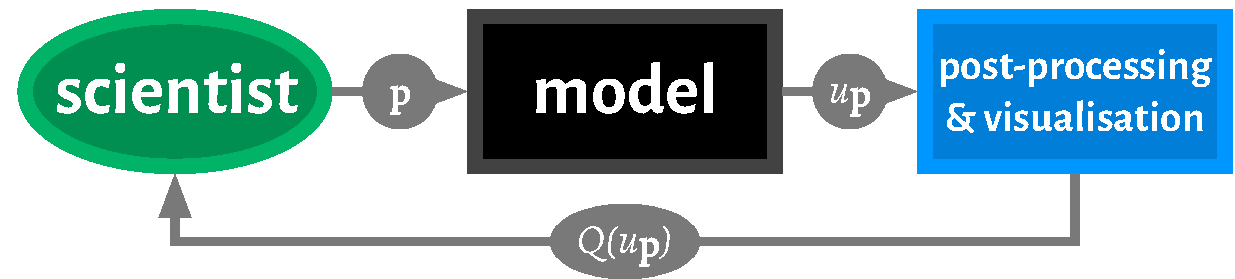
\includegraphics[width=.75\textwidth]{figures/general-fb-loop.pdf}
  \caption{The modelling workflow. A scientist selects an initial
    parameter $\mathbf{p}$ for their model, examines the model output
    $Q(u_{\mathbf{p}})$, and either accepts the output of the model
    or re-runs the model with a different choice of the parameter
    $\mathbf{p}$.}
  \label{fig:general-fb-loop}
\end{figure}

There are many ways of finding the optimal $\mathbf{p}$, from trial
and error or expert judgements through to fully automated algorithmic
optimization procedures (providing both $Q(u_{\mathbf{p}})$ and
$Q(u_{\mathbf{p}})$ are sufficiently nice, although this is often not
the case in real-world problems). Often there are some parameters
which may be optimised algorithmically, although this often introduces
new parameters (the inputs to the optimisation algorithm) which must
be selected by the scientist. As a result, this feedback loop will
often require many iterations, with a human scientist evaluating the
results of the model (possibly through visualising the model output)
and choosing a parameter update $\delta p$ at each step (see
Figure~\ref{fig:unrolled-fb-loop}).

\begin{figure}
  \centering
  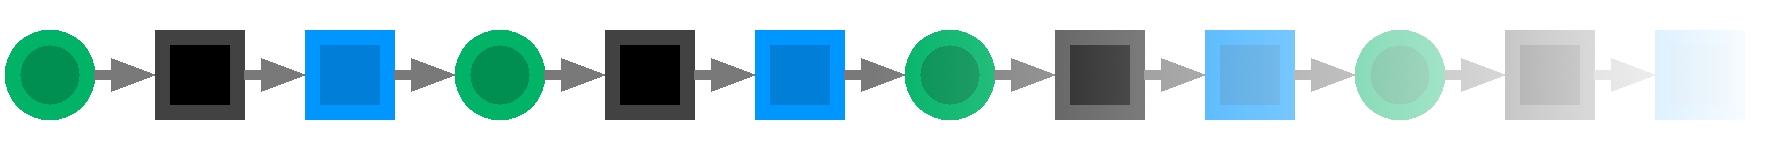
\includegraphics[width=\textwidth]{figures/unrolled-fb-loop.pdf}
  \caption{This process may require many iterations.}
  \label{fig:unrolled-fb-loop}
\end{figure}

For a given $\mathbf{p}$, the
scientist applies the model, updates their understanding of the system
based on the computed $Q(u_{\mathbf{p}})$, and potentially adjusts
$\mathbf{p}$ and continues the process. This process of ``twiddling
the knobs to find the parameters which give the desired outcome''
occupy a large part of the scientists and/or domain experts time.

From a workflow perspective, the productivity of the scientist is
proportional to the rate at which they can explore the
$\mathbf{p} \rightarrow Q(u_{\mathbf{p}})$ relationship. Any latency
improvements in this feedback loop will translate into
productivity gains\todo{ref}.
% With a tight feedback loop a natural extension would be providing tools for exploring the $Q(u_{\mathbf{p}}) \rightarrow \mathbf{p}$ relationship.

If the model parameters $\mathbf{p}$ and inputs $\mathbf{x}$ are known
precisely and the quantity $Q(u_{\mathbf{p}})$ is cheap to calculate
and easy to interpret, then the task is simple: provide the scientist
with an interface for manipulating $\mathbf{p}$ and set them loose.
However, for real-world models (such as those used in flood scenario
modelling?) this is often not the case, for the following reasons.
\todo[inline]{rather than the generic appeal to ``in the real
  world\ldots'', we could say ``we limit our analysis to situations
  where''\ldots}
\begin{enumerate}
\item \emph{The model may not provide a way to express uncertainty in
    the inputs}. Many models do not provide methods for including
  uncertainty information in their inputs, as was the case in the
  Lockyer valley example.@
\item \emph{The quantity $Q(u_{\mathbf{p}})$ may not be cheap to
    calculate} (as shown in Figure~\ref{fig:long-fb-loop.pdf}). Many
  sophisticated models require non-trivial computing resources to
  evaluate, such as supercomputers. These compute resources may be
  difficult to secure, with jobs having to wait in a queue, and may
  take a long time to compute even when the resources are available.
\item \emph{The quantity $Q(u_{\mathbf{p}})$ may not be easy to
    interpret}. This may be because of technical reasons, such as a
  complex problem domain where coming up with a meaningful loss
  function is difficult, or may be due to ethical reasons---how to
  balance the predicted cost to private property vs damage to the
  natural environment. Finally, this is a visualisation problem---
  the mapping $\mathbf{p} \rightarrow Q(u_{\mathbf{p}})$ may be high-dimensional,
  and presenting that to the scientist (especially with uncertainty
  information) may not be straightforward.
\end{enumerate}
\begin{figure}
  \centering
  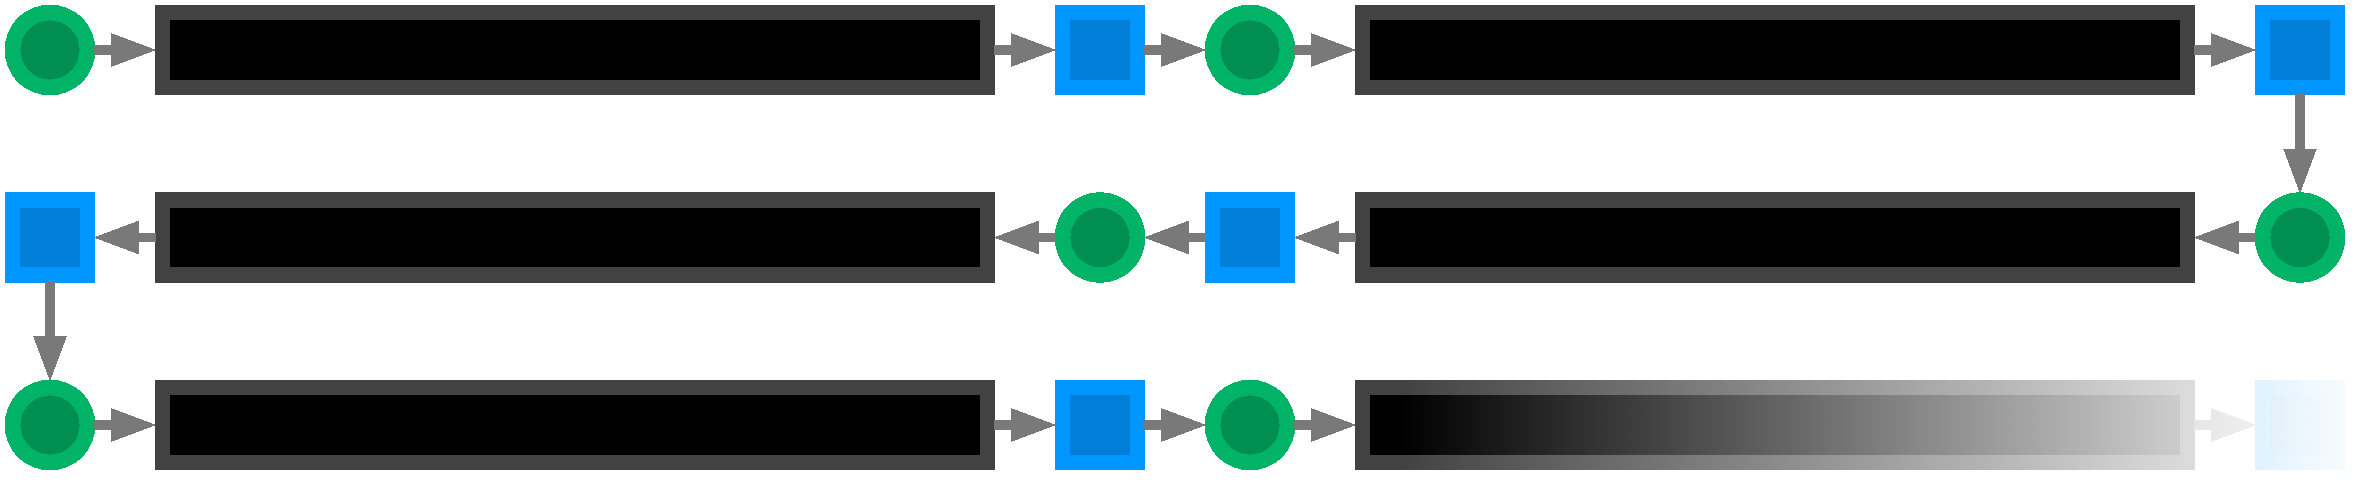
\includegraphics[width=\textwidth]{figures/long-fb-loop.pdf}
  \caption{If the model is computationally expensive to run, then the
    workflow is dominated by waiting for the model to finish. This
    results in lower productivity---not only due to the time spent
    waiting for the model, but also because of the temporal separation
  between the selection of a new parameter $\mathbf{p}$, and seeing
  its impact on the results of the model.}
  \label{fig:long-fb-loop.pdf}
\end{figure}
By accelerating the feedback loop between $\mathbf{p}$ and
$Q(u_{\mathbf{p}})$, including estimates of uncertainty, we will give
the scientist the ability to interactively \emph{explore} the
connection (and the associated uncertainty) between the different
dimensions of $\mathbf{p}$ and the overall response of the
system.

Ultimately, the scientist needs \textbf{interactive interface} for
gleaning insights from their models in the presence of these
challenges. Designing such a tool breaks down into two subtasks:
\begin{enumerate}
\item performing the modelling step
  $\mathbf{p} \rightarrow u_{\mathbf{p}}(\mathbf{x}) \rightarrow
  Q(u_{\mathbf{p}})$ sufficiently quickly for interactive exploration,
  while still providing adequate fidelity (including uncertainty). In this project, we will
  achieve this using \textbf{sparse grids} and \textbf{reduced basis
    models}.\todo{to what extent should we mention both SGs and RBMs?} %Probably SGs more than RBMs?
\item Presenting the quantities $\mathbf{p}$,
  $u_{\mathbf{p}}(\mathbf{x})$ and $Q(u_{\mathbf{p}})$ to the
  scientist, and take interactive input/parameter updates, in a way
  which provides meaningful insight. In this project, we will achieve
  this with \textbf{interactive scientific workflow management systems
    (SWfMS)}.\todo[inline]{we don't have to go the whole hog and talk
    about SWfMS, we could just call them interfaces, or interactive
    environments. Pros and cons to each. I guess the idea of using the
    SWfMS moniker is to tie it into existing research, and the call
    for full-stack SWfMS is loud in SoftEng at least.}
\end{enumerate}
\begin{figure}
  \centering
  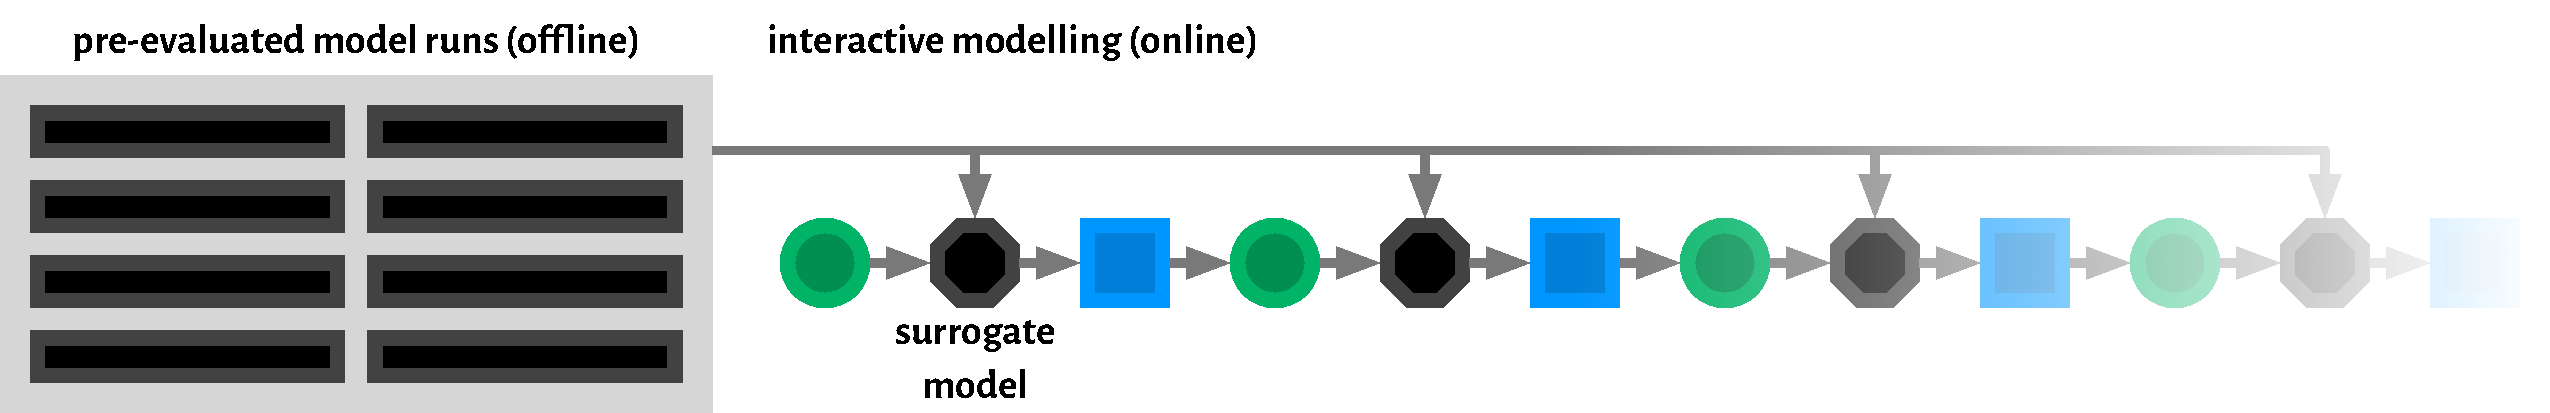
\includegraphics[width=\textwidth]{figures/sg-surrogate-model-fb-loop.pdf}
  \caption{If the model is computationally expensive to run, then the
    workflow is dominated by waiting for the model to finish. This
    results in lower productivity---not only due to the time spent
    waiting for the model, but also because of the temporal separation
  between the selection of a new parameter $\mathbf{p}$, and seeing
  its impact on the results of the model.}
  \label{fig:sg-surrogate-model-fb-loop.pdf}
\end{figure}
\todo[inline]{if we're going to say that interactivity is necessary
  (or at least extremely beneficial) then we need to make a case for
  it. I think we can, and it goes like: dealing with uncertainty
  requires the ability to explore, and exploration is \emph{heaps}
  better with a fast feedback loop, so interactive IO is
  necessary(ish). But if we decide that we don't want to make such a
  strong claim, we don't have to put this stuff in here.}

\missingfigure{full diagram of the scientist, the modelling steps and
  the relevant IO in an interactive feedback loop}

\subsubsection*{RESEARCH PROJECT}
% - Describe how the research is significant and how it addresses an important problem
% - Describe how the Proposal meets the objectives of the Discovery Projects scheme
% - Describe how the anticipated outcomes will advance the knowledge base of the discipline and
%   how the Proposal aims and concepts are novel and innovative
% - Outline the conceptual framework, design and methods and demonstrate that these are
%   adequately developed, well integrated and appropriate to the aims of the Proposal. Include
%   research plans and proposed timelines
% - Detail what new methodologies or technologies will be developed in the course of the research
%   and how they will advance knowledge
% - Outline the feasibility of the project, in terms of design, budget and proposed timeline
% - If the rationale for some of the Proposal rests upon manuscripts that are still in the process of
%   being published, or on results of work that may not be available to assessors, include a
%   summary of the relevant work
% - Describe the expected outcomes and likely impact of the proposed research
% - Describe how the Proposal might result in national or international economic, commercial,
%   environmental, social and/or cultural benefits
% - If the research has been nominated as focussing upon a topic or outcome that falls within one
%   of the Science and Research Priorities, describe the potential for the project to contribute to the associated Priority Goals.

There are two opposite, and equally unhelpful, ways of dealing with
uncertainty in modelling. The first is to ignore it, and assume that
the inputs to our models are known exactly. While this approach can be
(and indeed is) used when the uncertainties involved are small,
increasingly complex models means increasingly complex interactions
between the different parameters, and so it very difficult to say
which uncertainties are ``small enough'' to ignore. The opposite
approach is to \emph{ignore} input data about which there is too much
uncertainty. While this is a more conservative approach, it too can
lead to real problems, as in the 2011 Brisbane floods.

\paragraph{Sparse grids (and reduced basis models as well?)}

\todo[inline]{Brendan will beef up this section with lots of tricky
  maths which makes us sound smart. But it's very much a
  work-in-progress at the moment.}

In this project we will use sparse grid 
techniques~\parencite{BungartzGriebel2004} \todo{more refs?}
to approximate the model solutions $\tilde{u}_{\mathbf{p}}(\mathbf{x})$.
Sparse grids are well-known to reduce the effects of the so called 
`curse of dimensionality', whereby the cost of computation increases 
exponentially with the dimension of the model. 
For example, discretising $[0,1]^{d}$ such that there are $m$ points in each dimension leads to $m^{d}$ points whereas a sparse grid approximation uses only $\mathcal{O}(m\log(m)^{d-1})$ points whilst only increasing error by a factor $\mathcal{O}(\log(m^{-1})^{d-1})$.
This is achieved by representing the discrete approximation of functions in a hierachical manner and throwing away the contributions which are small relative to the amount of computation involved.
The combination technique~\parencite{Griebel1990} is a method of computing sparse grid solutions without the need of working with directly with the hierarchical basis.
When we refer to computing with sparse grids in what follows we typically mean via the combination technique.

There are two ways in which classical sparse grid methods can benefit this 
project:
\begin{enumerate}
\item For many problems the computation of solutions 
$u_{\mathbf{p}}(\mathbf{x})$ to the model $M_{\mathbf{p}}$ can be done 
cheaply using the combination technique over the domain $\mathbf{x}\in\Omega$,
\item A sparse grid sampling of $\mathbf{p}\in\mathcal{P}$ enables a fast 
and efficient exploration of parameter space. This can be approached in an online/offline approach.
\end{enumerate}

\begin{figure}[h!]
\centering
% Brendan: combination grid, sparse grid, fullgrid figure

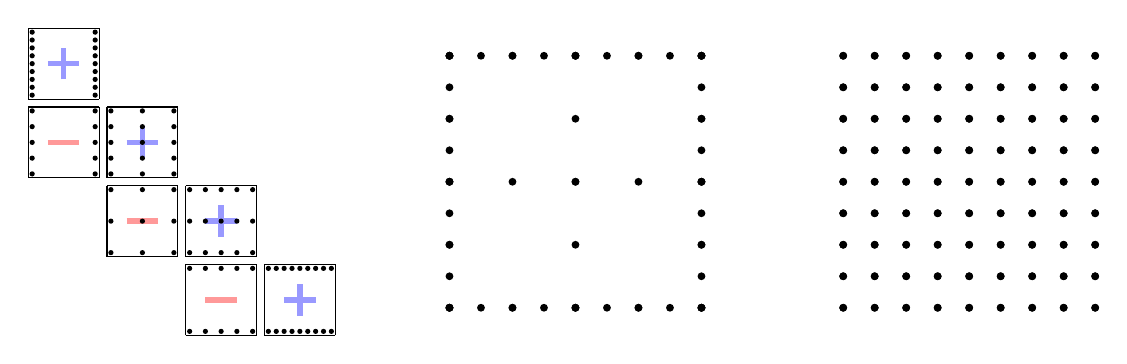
\begin{tikzpicture}%[scale=0.8]
%\scriptsize
%%% Draw squares around component grids
\foreach \i in {1,...,4}
{
	\pgfmathtruncatemacro{\x}{(\i - 1)};
	\draw[] (0.05+1.0*\x, 3.05-1.0*\x) -- (0.05+1.0*\x+0.9, 3.05-1.0*\x) {};
	\draw[] (0.05+1.0*\x, 3.05-1.0*\x) -- (0.05+1.0*\x, 3.05-1.0*\x+0.9) {};
	\draw[] (0.05+1.0*\x+0.9, 3.05-1.0*\x) -- (0.05+1.0*\x+0.9, 3.05-1.0*\x+0.9) {};
	\draw[] (0.05+1.0*\x, 3.05-1.0*\x+0.9) -- (0.05+1.0*\x+0.9, 3.05-1.0*\x+0.9) {};
	%%% optional plotting of coefficients
	\draw[blue!40,line width=0.7mm] (0.5+1.0*\x-0.2, 3.0+0.5-1.0*\x) -- (0.5+1.0*\x+0.2, 3.0+0.5-1.0*\x);
	\draw[blue!40,line width=0.7mm] (0.5+1.0*\x, 3.0+0.5-1.0*\x-0.2) -- (0.5+1.0*\x, 3.0+0.5-1.0*\x+0.2);
}
\foreach \i in {1,...,3}
{
	\pgfmathtruncatemacro{\x}{(\i - 1)};
	\draw[] (0.05+1.0*\x, 2.05-1.0*\x) -- (0.05+1.0*\x+0.9, 2.05-1.0*\x) {};
	\draw[] (0.05+1.0*\x, 2.05-1.0*\x) -- (0.05+1.0*\x, 2.05-1.0*\x+0.9) {};
	\draw[] (0.05+1.0*\x+0.9, 2.05-1.0*\x) -- (0.05+1.0*\x+0.9, 2.05-1.0*\x+0.9) {};
	\draw[] (0.05+1.0*\x, 2.05-1.0*\x+0.9) -- (0.05+1.0*\x+0.9, 2.05-1.0*\x+0.9) {};
	%%% optional plotting of coefficients
	\draw[red!40,line width=0.7mm] (0.5+1.0*\x-0.2, 2.0+0.5-1.0*\x) -- (0.5+1.0*\x+0.2, 2.0+0.5-1.0*\x);
}
%%% Combination grids
\foreach \i in {1,...,18} %2*9
{
	\pgfmathtruncatemacro{\y}{(\i - 1) / 2};
	\pgfmathtruncatemacro{\x}{\i - 1 - 2 * \y};
	\node[fill,circle,scale=0.2] at (0.1+0.8*\x,3.1+0.1*\y) {};
	\node[fill,circle,scale=0.2] at (3.1+0.1*\y,0.1+0.8*\x) {};
}
\foreach \i in {1,...,15} %3*5
{
	\pgfmathtruncatemacro{\y}{(\i-1)/3};
	\pgfmathtruncatemacro{\x}{\i-1-3*\y};
	\node[fill,circle,scale=0.2] at (1.1+0.4*\x,2.1+0.2*\y) {};
	\node[fill,circle,scale=0.2] at (2.1+0.2*\y,1.1+0.4*\x) {};
}
\foreach \i in {1,...,10} %2*5
{
	\pgfmathtruncatemacro{\y}{(\i-1)/2};
	\pgfmathtruncatemacro{\x}{\i-1-2*\y};
	\node[fill,circle,scale=0.2] at (0.1+0.8*\x,2.1+0.2*\y) {};
	\node[fill,circle,scale=0.2] at (2.1+0.2*\y,0.1+0.8*\x) {};
}
\foreach \i in {1,...,9} %3*3
{
	\pgfmathtruncatemacro{\y}{(\i - 1) / 3};
	\pgfmathtruncatemacro{\x}{\i - 1 - 3 * \y};
	\node[fill,circle,scale=0.2] at (1.1+0.4*\x,1.1+0.4*\y) {};
}
%%% Sparse grid
\foreach \i in {1,...,18} %2*9
{
	\pgfmathtruncatemacro{\y}{(\i - 1) / 2};
	\pgfmathtruncatemacro{\x}{\i - 1 - 2 * \y};
	\node[fill,circle,scale=0.3] at (5.4+3.2*\x,0.4+0.4*\y) {};
	\node[fill,circle,scale=0.3] at (5.4+0.4*\y,0.4+3.2*\x) {};
}
\foreach \i in {1,...,15} %3*5
{
	\pgfmathtruncatemacro{\y}{(\i-1)/3};
	\pgfmathtruncatemacro{\x}{\i-1-3*\y};
	\node[fill,circle,scale=0.3] at (5.4+1.6*\x,0.4+0.8*\y) {};
	\node[fill,circle,scale=0.3] at (5.4+0.8*\y,0.4+1.6*\x) {};
}
%%% Full grid
\foreach \i in {1,...,81} %9*9
{
	\pgfmathtruncatemacro{\y}{(\i - 1) / 9};
	\pgfmathtruncatemacro{\x}{\i - 1 - 9 * \y};
	\node[fill,circle,scale=0.3] at (10.4+0.4*\x,0.4+0.4*\y) {};
	\node[fill,circle,scale=0.3] at (10.4+0.4*\y,0.4+0.4*\x) {};
}
\end{tikzpicture}
\caption{Combination grids on the left (with coefficients, blue plus for $+1$ and red minus for $-1$), sparse grid in the middle, full grid on the right.}
\end{figure}


Much recent work with sparse grids has shown that the methods and ideas
from the classical work can be applied in other ways.
For example, sparse grids and related ideas have been used for
\begin{itemize}
\item fault tolerant computing~\cite{HardingHLS2015,AliEtal2015}
\item development of highly scalable algorithms~\cite{StrazdinsEtal2015}
\item gradient-enhanced approximation methods~\cite{deBaarHarding2015,Jakeman2015}
\item multi-fidelity approximation (similar to~\cite{deBaarRDM2015}) 
\item solution of large scale inverse problems~\cite{Zabaras2010}
\item uncertainty quantification~\cite{JakemanRoberts2013,FranzelinDiehlPfluger2014}
\item reduced basis methods~\cite{Peherstorfer2013,ChenSchwab2015}
\end{itemize}
We envisage this project making full use of these advances in addition 
to the classical approaches with the end goal of providing fast, accurate
and robust approximations of model solutions to scientists whilst 
incorporating all of the uncertainties in the underlying model and its inputs. 
Achieving this goal will require further research and development.
We expand on some of these points in the remainder of the section.

One of the problems often faced by scientists is having too many models 
to choose from. On top of this, for each model there are typically numerous
numerical methods for approximating solutions of the model.
This leads to the all too common question `what is the `best' model and alorithm?'.
Naturally `best' depends on the criteria but typically no one model/algorithm is
the `best' for all selection criteria.
Gradient-enhanced and multi-fidelity approximation and similar ideas give one
the ability to combine some of the `best' attributes from several methods into one approximation.
This potentially leads to a more accurate result and more generally a much better
understanding of the models and their relation to the physical problem under investigation.
Of course the problem is that managing and evaluating several methods is time
consuming. By making such tools available in a highly interactive environment
such exploration will become more accessible. With accessibility comes higher 
uptake leading to significant gains in understanding for a variety of problems.

Many of the models used in modern science require high performance computing
to approximate solutions. Much work has gone into the development 
of highly scalable sparse grid algorithms, specifically using the combination 
technique, which this project will utilise and continue to develop. 
One challenge is that faults become more frequent with increasing 
complexities in computing hardware and ever more components essential 
for a HPC system to function correctly. Fortunately, there has been much interest in 
fault-tolerance recently and, in particular, the development of fault tolerant 
sparse grid methods. By leveraging this work into our framework we can ensure
accurate results even in the event of some data being lost during the computation.
Prior reseach has focused on recovery from hard faults. Whilst some studies are
being conducted into recovery from silent errors there is more research to be done in this area.
More generally, having a framework which is robust to errors increases the confidence 
in the results and therefore also the decisions which are based on those results.

Sparse grids are typically applied to uncertainty quantification in the
estimation of high dimensional integrals (to estimate expectations for example). 
For sufficiently smooth probability density functions sparse grids provide
an accurate estimate using far fewer function evaluations then the Monte Carlo 
method.
This approach also suits an offline-online model of computation.
Given a sparse grid sampling/surrogate computed in an offline phase, high 
dimensional integrals, including the estimation of moments of a probability distribution,
can be quickly and accurately estimated in an offline phase.
Additionally, there is potential to extend existing work in this area. 
In particular, the addition of gradient estimates and multi-fidelity models 
to the sparse grid surrogate, 
the extension to a more probablistic sparse grid model (akin to kriging) and
and how each of these enhance the quantification of uncertainty will be investigated.
% Examples? Any snappy quotes from the refernces I can use?

%in ways which are:
%\begin{enumerate}
%\item able to express and propagate uncertainty in both input
%  parameters and outputs
%\item cheap to calculate, so that these approximations can be explored
%  in a real-time human-in-the-loop exploratory workflow
%\end{enumerate}
%As an added bonus, these general techniques can be used to quantify
%the uncertainty in models (or ensembles of models) even when the
%models themselves were not designed with uncertainty quantification
%(UQ) in mind \todo{in the parameter space, anyway---Brendan, is this
%  the ``smarter monte carlo'' stuff you were talking about the other
%  day?}, and to combine multiple models (e.g. high- and low-fidelity
%models) in a sophisticated way to leverage the benefits of many
%different models.


There has been much interest in reduced basis methods to make large
problems more tractible~\cite{LiebermanEtal2010}. %\todo{more refs?}

Reduced basis methods could have several applications to this project.
The computation of a reduced basis model in an offline phase
will allow a scientist to quickly explore the parameter space in an online
phase.
Further, a reduced basis model may allow a scientist to learn more about the 
the inverse problem of finding the parameters $\mathbf{p}$ that lead to a 
given output $Q(u_{\mathbf{p}})$.
There are several opportunities to continue developing the application 
of sparse grid methods to reduced basis construction which would be
fully integrated into the interactive scientific workflow management system.


%Recent work on sparse grid techniques is finding new ways to
%combine results from not only mathematical models computed via
%different methods \todo{Brendan add refs to sparse grid extrapolation
%techniques} but also entirely different mathematical
%models \todo{Brendan add refs to Jouke et.al. work on ship hull with 2
%models}. It is clear that different methods and models
%have their own advantages and disadvantages which have the potential
%to be combined in new and interesting ways. [Point trying to make: a)
%the usual 'too many methods' dilemma, and b) there is generally no one
%'best' method and yet it is typical to pick one and stick with it
%(based on some comparison with others)]

%Of course the difficulty is that such exploration is time consuming
%and can be difficult to keep track of. By combining all of these
%methodologies and techniques into a single framework one may more
%easily test and combine the vast number of different approaches to
%solving any given problem. Further, by implementing this within an
%interactive/live programming environment, users can quickly adjust methods
%and parameters as needed whilst getting near instant feedback and
%response. Such tools could significantly increase the speed at which
%research is undertaken and allow us to learn more from our
%mathematical models than previously envisioned.

This section will also include the offline/online stuff, and the
flexible cloud infrastructure stuff as well.

\paragraph*{Building interactive systems for exploring uncertainty relationships}\mbox{}\\

\todo[inline]{We have some stuff to use here (see content on page
  \pageref{SWfMS-grant}), but it needs some work to be successfully
  integrated.}

% Why is interactivity important? Because it takes the abstract
% connection between $\mathbf{p}$ and $Q(u_{\mathbf{p}})$ and makes it a malleable,
% responsive, tactile one. What happens when I change $\mathbf{p}$ a little bit
% in this direction? What about in \emph{that} one? How about \emph{both
%   together?}

\subsubsection*{ROLE OF PERSONNEL}
% - Summarise the role, responsibilities and contributions of each Chief Investigator (CI) and Partner Investigator (PI)
% - Summarise the roles and levels of involvement of other Participants, for example, technical staff, Research Associates and other personnel
% - Describe how each Participant will ensure they have the ‘time and capacity’ to undertake the proposed research, taking into account any other grants or roles that they hold.

The personnel on this grant cover the key research areas discussed in
the \emph{Research Project} section of this application:

\begin{itemize}
\item \textbf{Steve Roberts}: uncertainty quantification, sparse grids, flood
  modelling
\item \textbf{Markus Hegland}: sparse grids
\item \textbf{Peter Strazdins}: sparse grids, distributed computing
\item \textbf{Henry Gardner}: HCI, interfaces
\end{itemize}

\subsubsection*{RESEARCH ENVIRONMENT}
% - Outline the adequacy and opportunities within the Research Environment in your relevant department, school or research group, and the extent to which it will provide for knowledge growth, innovation, collaboration, mentoring and student training
% - Describe the existing, or developing, research environment within the Administering Organisation and collaborating Organisation(s) which will enable this Project
% - Describe how the Project aligns with the Administering Organisation’s research plans and strategies.

\todo[inline]{I'm open to suggestions on how to pitch the ``research
  environment'' section from those more experienced at getting money
  out of the ARC than I}

It seems we need to address three issues: 

\begin{enumerate}
\item the environment within the department/school/research group
\item the environment between the groups---perhaps between the MSI
  group and the CS group, (and also CSIRO?)
\item how does it align with the ANU's research plans and strategies
\end{enumerate}

Ideas\ldots

Numerical methods and applied mathematics---we're kicking goals.

Collaboration across maths and compsci, have track record through e.g.
the Fujitsu grant

CSIRO/ADFA/BOM(? although we haven't mentioned them thus far) for more
fire and flood stuff

\subsubsection*{COMMUNICATION OF RESULTS}
% - Outline plans for communicating the research results to other researchers and the broader community, including but not limited to scholarly and public communication and dissemination.



\subsubsection*{MANAGEMENT OF DATA}
% - Outline plans for the management of data produced as a result of the proposed research, including but not limited to storage, access and re-use arrangements.
% - It is not sufficient to state that the organisation has a data management policy. Researchers are encouraged to highlight specific plans for the management of their research data.



\subsubsection*{REFERENCES}

\vskip -3em
\printbibliography[title=\ ]

\appendix
\newpage

\todo[inline]{Ok, from here on it's the wild west. Caveat lector.}

\textbf{Ben notes}: uncertainty and risk in decisionmaking - it's a
real problem that bites

BNE floods were in part a human factors problem - they decided to make
decision based on ignorance rather than uncertainty

fire: The myriad of information collected from diverse sources had a broad
range of reliability---\parencite{cruz_anatomy_2012}

\blockquote[\parencite{alexander_limitations_2013}]{Given the nonlinear
  dynamics of free-burning wildland fires (Sullivan 2009d), model
  output may be highly sensitive to a particular parameter over one
  range of values and quite insensitive to that same parameter over a
  different value range (Albini 1976a, Cruz et al. 2006)}

but one other limitation is the modelling is just provided - limited
ability to assess different scenarios other than the ones presented,
and therefore unable to do the helpful ``relative/anchoring'' natural
decisionmaking approach which is what actually happens in these
scenarios

\blockquote[\parencite{vandenhonert_2011_2011} p1158]{In the aftermath of
  the January 2011 flood, a senior Wivenhoe engineer has stated before
  the Commission of Inquiry [17] that uncertainty in BoM rainfall
  forecasts and the paucity of rain gauges in the catchment
  immediately above the Wivenhoe Dam led them to conclude that the
  precipitation forecasts were not sufficiently reliable to form the
  basis for operational decision making.}

naturalistic decisionmaking\parencite{lipshitz_taking_2001}

Can we make the case that the better approach to the uncertainty thing
is the constructivist one? need some refs I reckon


uncertainty and complexity are present and irreducible. human factors!

human in the loop (or something similar) is generally accepted

but all the papers making a big deal of that gloss over the technical
challenges of this + complex models

\textbf{Notes from Henry}: important in the project proposal is to identify the
potential ``discoveries''. What are they and how to they motive
funding?

\begin{enumerate}
\item a suite of interactive, real-time modelling tools which combine
full simulations with coarse-grid, rough simulations to quantify
uncertainty, optimised for human use
\item software support for running these simulations in unpredictable
and error-prone environments
\item interactive information visualisations of simulation predictions
together with uncertainty
\item an agile software engineering approach to the further delopment
and optimisation of these software systems
\end{enumerate}

The proposal needs to document the methodology to be followed. I think
that this could include:

\begin{enumerate}
\item construction of a virtual command room
\item construction of a prototype suite of modelling software
\item interviews with domain experts from Geosciences, Flood
  management, RFT
  \begin{enumerate}
  \item from these interviews, develop principal distraction scenarios
    to be tested in the virtual command room
  \item build a form of cooperative game that would be played by a
    group of test participants
  \end{enumerate}
\item development and testing of interactive visualistions
\end{enumerate}

What this proposal does NOT include is advice from AI agents. That can
be left to others in collaboration with us.

At present, the version of the proposal that I have seen has a focus
on flood modelling. I wonder if we could better position it in the
realms of storm surges. Important for the future. Links to bathymetry
and tsunamis etc. What do people think?

% overview of dynamic decision support
% systems\parencite{gonzalez_decision_2005}

% mceachern on the current SoA in visual analytics and
% uncertainty\parencite{maceachren_visual_2015}

% \textquote[\parencite{sprague_framework_1980}]{interactive computer
%   based systems, which help decision makers utilize data and models to
%   solve unstructured problems.}

\textcite{zack_role_2007} describes four classes (well, $2\times2$ really) of uncertainty:
\begin{itemize}
\item Uncertainty: not having enough information;
\item Complexity: having more information than one can
\item Ambiguity: not having a conceptual framework for interpreting
  information;
\item Equivocality: having several competing or contradictory
  conceptual frameworks.
\end{itemize}

In addition, recent developments in sensor networks and pervasive
monitoring technologies have increased our ability to gather data from
the world. Streaming data analysis is an active area of research, and
in an uncertainty quantification context streaming data provides the
opportunity to be continuously estimating model uncertainties and
updating our models in response to new data coming in.

This project asks the question: \textbf{can streaming data be used to
  update and model uncertainties and provide intelligible insights in
  time-critical decisionmaking scenarios?}

One example scenario: sensors detect an earthquake in the Pacific Ocean,
and the countdown timer begins---what is the likelihood of a
destructive tsunami, where will it impact, and does an evacuation
order need to be issued? Some initial modelling has already been done,
but new readings are coming in regularly from sensor buoys throughout
the ocean. How can this new (and potentially noisy) data be used to
update the model, and how does this affect the predicted impact? How
does uncertainty in the buoy readings affect our confidence in the
model?

\todo[inline]{What follows is from a draft which Henry and Ben started
to put together last year, and there is some material here which could
be used to fill out the ``building the interfaces'' part of the
``Research Project'' section of this application. But it won't
necessarily make sense as-is.}

\subsubsection*{AIMS AND BACKGROUND}
\label{SWfMS-grant}
\paragraph*{Aims}\mbox{}\\

The modern world appears to be saturated with computing power.
Contemporary smart phones outperform the original Cray~1
``supercomputer'' by three orders of magnitude. Accessing contemporary
high-performance computing (HPC) resources has never been easier and,
when combined with machine learning\parencite{Hastie2009}, and big
data\parencite{Manyika2011}, modern supercomputing performance has the
potential to provide answers to deep questions in science, business
and the humanities.

Modern comodity computing devices are spectacularly \textbf{visual}
and \textbf{interactive}, enabling users to slide, tap, watch, speak
and listen with real-time feedback. It is this combination of
interactivity with power which makes mobile and personal computing
useful, usable and an agent of change.

But the closer one comes to true high-performance computing, the less
interactive computing systems become. Due to a combination of
technical and social factors, high-performance scientific computing
(HPSC) is still often performed in a batch \emph{compile-run-analyse}
style: simulation codes are complex both conceptually (i.e.~the
underlying mathematics and physics) and in implementation (distributed
computation, large codebases). Supercomputing resources are expensive
and need to be kept secure.

It is worthwhile imagining some example scenarios that might be
possible if better interactive \textbf{access to} and \textbf{steering
  of} scientific supercomputing applications were to be available:
\begin{enumerate}
\item A computational physicist submits a job to a supercomputer which
  takes 3 weeks to execute. But subsequent monitoring of incremental
  visualisations indicates that something about the simulation does
  not make sense.A check of the, almost 200, input parameters reveals
  that two of these have been incorrectly set. The phyicist cancels
  this run and submits another.

\item That same physicist has a sudden insight into the physical
  system being modelled as a result of watching some of the
  incremental visualisations of the running code. She initiaties a new
  simulation with several changes to the parameter deck before the
  first simulation is complete. Both simulations turn out to be useful
  in understanding the phenomenon under study.

\item Our physicist decides to improve the numerical accuracy of the
  model itself. She quickly modifies one of the functions being called
  by that simulation, one that implements flux-conservation across
  computational elements of the magneto-fluid being modelled. She then
  tests her new function on the active program by branching the
  simulation and swapping the function call on active data. Through a
  comparison of the two active simulations, she is able to estimate
  what the effects of her new numerical method will be on the
  accumulation of errors in the simulation data. She lets both
  simulations run to completion, and in her subsequent data analysis,
  she is able to use her error estimates to adjust and compare
  sumulations using both methods.

\item Performance diagnostics reveal that a multicore simulation is
  very unbalanced in terms of processor allocation. Due to the
  complexity of this simulation, the only way to rebalance resources
  is to rewrite part of the code which maps the geometric grid to the
  processor model. Our physicist is able to rewrite this function and
  to swap the new version in, in real-time. The simulation continues
  seemlessly with enhanced use of resources and finishes faster.

\item A computer scientist is developing a custom visualisation of a
  scientific simulation. Because of the size of the dataset being
  rendered, and because of its distribution across hundreds of
  processors it is impossible to move all of the data. Instead each
  data nodes needs to be ``visited'' and a sample of that data
  transferred for visualisation. This visualisation is planned, tuned
  and debugged on running code and is complete by the time actual the
  simulation is finished.

 % \item A bioinformatics researcher runs a supercomputer simulation which searches and matches millions of generated phylogenic candidates in order to develop evolutionary trees. Rather than 

%A subsequent analysis of the results finds that the stopping
%   criteria were satisfied after only the first hundered such files had
%   been compared.

\item A team of emergency-services personnel are monitoring a
  real-time satellite feed of a bushfire which is hours away from
  threatening homes and lives. A computational simulation of the
  bushfire is being monitored and compared with data but it appears to
  be giving unreliable results. The simulation experts quickly
  initiate several companion simulations having different values of
  fuel loads. The fire-front trajectories of these companion
  simulations neatly bracket those of the main simulation and provide
  an estimate of the confidence that can be ascribed to those
  predicted fire-fronts.


%\item A growing hi-tech manufacturing company has historically relied
%  on managing their supply chain by hand. However, as the company
%  grows and the number of supplier relationships increases this is no
% longer feasible. A purely automated approach generates suboptimal
%  results, because the supply chain involves a complex network of
%  human relationships and hand-shake agreements between the suppliers.
%  The expert team can see subtle problems with the results (and
%  appropriate subtle corrections) as the automated model is running,
%  but are prevented by the software from making these changes until
%  the model has finished running.
\end{enumerate}

All of these scenarios benefit from a tight human-in-the-loop (HIL)
coupling between run-time analysis, visualisation and high-performance
simulation software. The benefits include greater \emph{efficiency}
and greater \textbf{potential for discovery} in scientific workflows.
\textbf{The aim of this project proposal is thus to build
  human-in-the-loop interactivity into high performance scientific
  computing}.

\paragraph*{Background}\mbox{}\\

In 2007, a National Science Foundation (NSF)
workshop\parencite{Gil2007} highlighted the need for dynamic
interactivity as a looming ``grand challenge'' in scientific
computation and data analysis.
% Other challenges included data provenance (where data comes
% from\parencite{McPhillips2009}), reproducibility and shareability of
% complex data processing software pipelines.
In spite of many advances in the field of computational steering it is
clear that challenges remain. A recent (2014) review, ``Dynamic
steering of HPC scientific workflows: A survey''\parencite{Mattoso},
identified six key areas of interaction/steering:
\begin{enumerate}
\item \textbf{monitoring}: the ability to monitor intermediate
  quantities of interest (e.g.~total energy)
\item \textbf{analysis}: the ability to perform analysis of simulation
  quantities (e.g.~viewing a live histogram of the energy
  distribution)
\item \textbf{adaptation}: the ability to adapt/modify the running
  simulation
\item \textbf{notification}: the ability of the system to alert users of the
  need/opportunity to interfere
\item \textbf{interface for interaction}: the interface (either command-based
  or GUI) presented to the user to monitor and adapt the computation
\item \textbf{computing model}: the ability to tailor the types of interaction
  depending on the compute model in use (e.g.~providing full
  monitoring when running locally on a workstation vs only statistical
  sampling when the job is distributed over a cluster)
\end{enumerate}
At the end of their survey, Mattoso et~al.~particularly identify the
\emph{analysis} and \emph{adaptation} branches of their taxonomy as
not being well addressed by the current state of the art.

Elaborating further, in terms of \emph{real-time analysis} the open
challenges are:
\begin{itemize}
\item \textbf{in-situ analysis}: modern terascale compute
  infrastructure is often IO-bound, and HPC applications must minimise
  inter-node communication to achieve efficient use of the hardware.
  As a result, it is often unfeasible to move the data of interest
  back to a central node for processing and analysis, so any such
  analysis must be performed in-situ\parencite{Bennett2012} on the compute
  node itself.
\item \textbf{decision-support tools}: giving a user the
  \emph{ability} to interfere with a running computational process is
  one thing---knowing \emph{when and how} to interfere is another
  thing altogether. Dynamic SWfMS must provide as useful real-time
  feedback to the user (a domain expert) to assist them in deciding
  when and how to interfere. This problem is an example of a more
  general end-user programming (EUP)\parencite{Myers2006} problem---giving
  domain experts the appropriate tools to transfer their domain
  expertise into the computational domain.
\end{itemize}
In the area of \emph{adaptation} the open challenges are:
\begin{itemize}
\item \textbf{dynamic workflow engines}: most of the surveyed systems
  allowed the user to adapt the computation at a high level (e.g.
  add/delete subtasks). However, there was much less support for
  modifying the evolution of specific tasks (e.g.~swapping out
  low-level algorithms and tight-loops in computation). This level of
  adaptivity would allow for even more steering possibilities, but may
  exacerbate the problem of deciding when/how to interfere (although
  support for rolling back interventions would be helpful here).
\item \textbf{parameter slice exploration}: many scientific problems
  involve searching high-dimensional parameter spaces for optimal
  parameter configurations, and many algorithms exist for this task.
  However, there are some problems (e.g.~buisness informatics) where
  cost/loss functions are hard to articulate, and more traditional
  purely numerical optimization approaches tend to overfit or get
  stuck in local maxima. In these situations an expert domain user, if
  presented with appropriate feedback in real-time, may be able to
  recognise these type of convergence problems early on, and perform
  appropriate algorithmic and parameter adaptations to avoid the
  problem.
\end{itemize}

The authors of this project proposal contend that all of these
challenges can now be effectively investigated by deploying recent
developments in programming language systems, known as ``live
programming'' (LP), into the context of high performance scientific
simulation. Live programming is a term which has been used to denote
systems which support the direct intervention of the programmer in a
program's runtime state. It can be thought of as an extreme version of
just-in-time (JIT) programming where there is a direct correlation
between a program's representation and its execution. An example of
this is the visual language Self\parencite{Ungar1987} where each visual
element in the language is a directly programmable object. As the
ambition of LP systems has grown, these systems and languages
themselves have evolved to have access to clock-time and other
computer-system properties at a language level in order to, for
example, create, modify and interact with computer music and devices
in real time. Examples of the latter include the
Impromptu\parencite{Sorensen2005} and Extempore\parencite{Sorensen} languages
which one of the authors of this proposal has been working on and with
over several years.


\subsubsection*{RESEARCH PROJECT}

% explore $\rightarrow$ enliven $\rightarrow$ empower

% Want to bring the idea of ``liveness'' to HPC/big data software – allow
% developers to get rapid, incremental update of target data process
% algs ; allow developers to get near-instantaneous feedback on input of
% changes to outputs data via rich visualisations

% Want to leverage domain-specific visual languages to specify these big
% data analysis problems to enable end users a high-level, controlled
% environment c.f. R-type scripting, code, BI configs etc

% Want to leverage rich information visualisations to provide small
% snapshot and overall output understanding by end users

% << Worth a big picture ``concept diagram'' here >>

% The aim of this project is thus to invent a new approach to specifying
% and realizing data-centric software systems using live visual
% programming and data visualisation we break into specific aims:

% - SDL++ for data analytics
% - Live visual programming of data analytics - DSVLs
% - extempore -> live update of GPU/HPC/IR/ML algs etc
% - live visualisations of complex data analytics alg data for feedback,
%   output
% - evaluate effectiveness by apply to several exemplars e.g.~particles,
%   big data analysis, infoVis...

This project will allow domain experts to better harness the power of
computational simulation the in a safe and effective way by creating
tools and interfaces for \emph{interactive} computational simulation
and anaylsis. This involves integrating research and tools from the
domains where such computational analyses are used with insights from
human-computer interaction and software workflows.

Through a series of exemplar case studies in different domains, we
will unlock new ways to perform complex computation analyses through
three steps:

\begin{enumerate}
\item \textbf{explore}: first, by exploring the problem domain (and
  existing tools) of interest in conjunction with domain experts, do
  determine the dimensions of the domain which could most benefit from
  interactive, human-in-the-loop analysis
\item \textbf{enliven}: taking these modelling and simulation codes
  and providing new interfaces for real-time interaction---this is not
  just a matter of superficially wrapping these systems in a slick
  GUI, but requires a restructuring of codes which are designed with
  batch processing in mind to allow for meaningful interaction and
  feedback
\item \textbf{empower}: using a user-centred design approach, we will
  create appropriate interfaces (e.g.~graphical user interfaces) to
  empower these domain experts to unlock their expertise in
  interactive computational simulation
\end{enumerate}

\paragraph*{Research significance}\mbox{}\\


Computational simulation and modelling is ubiquitous in both academia
and industry, and its importance is growing. Large-scale basic physics
relies on computational simulation to probe the subatomic landscape;
the auto industry uses simulation extensively for calculating the
efficiency of new designs; and algorithmic pattern recognition and
recommendation has transformed the way we search (Google), shop
(Amazon), watch (Netflix).

However, performing these analyses increasingly requires specialised
computational skills such as high-performance and distributed
computing. There is a risk that the power of simulation is available
only to a HPC-literate elite, and to those rare experts who assimilate
both the domain knowledge and computing skills to access it, and to
interpret it's results.

This research is significant because it aims to unlock the power of
computational simulation for interactive use. Although we concentrate
our research on case studies from extant computational science, the
ultimate potential of this work is to eventually empower domain
experts from a broad range of areas to use the high-performance
computing power which is now available to them. We envision a future
where performing a complex particle physics simulation is as
interactive and \emph{alive} as flicking through photos on an iPad,
rather than a tedious ``queue up the job, come back a week later to
pore over a dump of the results'' process. This benefits not only
experts already working in that field, but also allows new researchers
(or even schoolchildren) to understand the behaviour of such systems
through interactive play rather than dry textbooks.

% Big data software, HPC software becoming massively important
% Development of both still rudimentary, limited use of ``liveness''
% concept in HPC/DSVLs to date (some in InfoVis). Many applications of
% our approach; a very enabling technology. Examples might include\ldots

\paragraph*{Advancing the knowledge base with innovation}\mbox{}\\

As highlighted by Mattoso et~al.\parencite{Mattoso}, there is a desire for
more dynamic interactivity in scientific workflows, but progress in
that area has been limited. This project will contribute to the
knowledge base by providing these dynamic workflows, allowing us to
answer open questions such as:

\begin{itemize}
\item how can interactivity most effectively be ``added'' to existing
  scientific workflows?
\item how can automated assistance/analysis be provided to the user to
  best guide their interaction?
\item how do other outstanding issues in scientific computation, such
  as data provenance, reproducibility, etc.~impact the interactive
  workflow?
\end{itemize}

% \begin{itemize}
% \item very limited use of ``liveness'' concept to date in BI, HPC, etc;
%   adding into these very novel
% \item limited DSVLs leveraged to date in these domains; enables end
%   users
% \item InfoVis well studied but specification low-level, limited;
%   enables greater generality
% \item running the concept of ``liveness'' through these: DSVLs <->
%   HPC/Big Data code <-> InfoVis
% \end{itemize}

\paragraph*{Conceptual}\mbox{}\\

Series of research problems to be solved:

\begin{enumerate}
\item Add ability to modify HPC/Big Data code while
  running---``liveness''
\item Invent set of DSVLs for specifying such applications
\item Use DSVLs to generate code / modify code (via 2, 1 above)
\item Specifying rich, live InfoVis solution for data processed (by 1
  above)
\item Evaluate effectivess on set of exemplars
\end{enumerate}

\newpage
\setcounter{section}{5} % E1.
\setcounter{subsection}{0}
\subsection{Justification of funding requested from the ARC for the
  duration of the Project}
\label{sec:funding-justification}
% (In no more than 5 A4 pages and within the required format fully
% justify, in terms of need and cost, each budget item requested from
% the ARC. Use the same headings as in the Description column in the
% budget at Part D of this Proposal. )



\newpage
% E2.
\subsection{Details of non-ARC contributions}
\label{sec:non-arc-contributions}
% (In no more than 2 A4 pages and within the required format, provide
% an explanation of how non-ARC contributions will support the
% proposed Project. Use the same headings as in the Description column
% in the budget at Part D of this Proposal. )


\newpage
\setcounter{section}{6}
\setcounter{subsection}{11} % F12. 
\subsection{Research Opportunity and Performance Evidence (ROPE)\\
  Recent significant research outputs and ARC grants (since 2005)}
\label{sec:recent-significant-outputs}
% (Please attach a PDF with a list of your recent significant research
% outputs and ARC grants most relevant to this Proposal (20 pages
% maximum). Please refer to the Instructions to Applicants for the
% required content and formatting.)



\newpage
% F13. 
\subsection{Research Opportunity and Performance Evidence (ROPE)\\
  Ten career-best research outputs}
\label{sec:ten-best-outputs}
% (Please attach a PDF with a list of your 10 career-best research
% outputs, with a brief paragraph for each output explaining its
% significance (5 pages maximum). Please refer to the Instructions to
% Applicants for the required content and formatting.)



\newpage
\setcounter{section}{7} % G1. 
\setcounter{subsection}{0}
\subsection{Research support from sources other than the ARC}
\label{sec:other-research-support}
% (For all participants on this Proposal, please provide details of
% research funding from sources other than the ARC (in Australia and
% overseas) for the years 2014 to 2018 inclusive. That is, list all
% Projects/Proposals/Fellowships awarded or requests submitted for
% funding involving the Proposal participants. Please refer to the
% Instructions to Applicants for submission requirements.)

% \section{Conclusion}
% \label{sec:conclusion}

% Please give us all the money, and we'll do amazing science.

\printbibliography[title=References]

\end{document}

% Local Variables:
% TeX-engine: xetex
% End:
